\chapter{Sign languages}\label{chapterone}
In this chapter, I will make some brief remarks on sign languages in general (Section \ref{signlanguagesintro}), about the role of non-manual markings (Section \ref{sectionnmms}), and present some basic facts about DGS (Section \ref{basicclausstructuredgs}). 
%\clearpage
%


\section{Sign languages}\label{signlanguagesintro}
In this section, I will briefly illustrate that sign languages are natural languages with complex grammatical structures obeying the same structural building principles as spoken languages. I will do this cursorily by way of exemplification and illustrate that both spoken and signed languages exhibit duality of patterning\is{duality of patterning|see{double articulation}}\is{double articulation} and that recursion is found in both types of languages---two features which have been  claimed to be universally found in natural languages (\citealt{martinet1949double}; \citealt{hockett1960origin}). It is nevertheless crucial to note that sign languages are similar to spoken languages in nearly every respect. For example, they serve the same communicative functions, can express meanings in the same way and at the same speed as spoken languages \citep{bellugi1972comparison}, they are naturally acquired by children given normal exposure to the language (e.\,g., \citealt{newport1985acquisition}), and are processed in the same brain regions as spoken languages (e.\,g., \citealt{emmorey2002language}). To date, 142 different sign languages with distinct lexicons and distinct grammars with an approximate number of 5\,000\,000 speakers have been documented \citep{simons2018ethnologue} although it can be assumed that there are more, perhaps between 300 and 400 different sign languages used all over the world \citep{zeshan2009sign}. That there are so many different sign languages in the world has to do with the fact that sign languages naturally evolve when a sufficient number of deaf people come together over a longer period of time (e.\,g., \citealt{kegletal1999creation}).

\subsection{The phonology of spoken and signed languages---duality of patterning}
\is{double articulation|(}
%Thus, sign languages are fully-fledged natural languages. 
While spoken languages are produced by manipulating the air stream flowing through the oral and nasal cavities with the speech organs (the lips, the teeth, the glottis, the tongue etc.), sign languages are produced by the hands, arms, the torso, the head, and the face. Both language types are thus produced by performing gestures with the body. In the case of spoken languages, sound waves hit the eardrums which are set into oscillation. In the case of sign languages, it is light waves which are transformed into electrical signals through receptors within the retina. Differences between sign and spoken languages like these are often referred to as differences in modalities. While spoken languages use the auditory-vocal modality, sign languages make use of the visual-gestural modality. 

While the two language types look very dissimilar on the surface, the structural principles underlying both are astonishingly similar \citep{sandler1989phonology,brentari1998prosodic}. In both modalities, a limited number of elements is used together with a limited number of rules to create an unlimited number of utterances. On the phonological level, for example, spoken languages combine a limited set of phonemes (or distinct features creating phonemes) which are by themselves meaningless to create morphemes carrying meanings (of course, this process is not unconstrained, but governed by phonotactic rules). This way of creating meaning is characteristic of human languages and called `duality of patterning' or `double articulation' \citep{martinet1949double, hockett1960origin}.

In both language types it is possible to create two morphemes that differ in only one feature, i.\,e., to create minimal pairs showing that the two features indeed belong to the set of relevant building blocks of the language. In English, the (monomorphemic) words \textit{cool} and \textit{tool}, for example, only differ in place of articulation of its initial plosive. From this, we can not only infer that the plosives /k/ and /p/ are phonemes of English, but also that the velum (the soft palate) and the alveoli (the tooth sockets) are places of articulation in English used as distinctive features. The same process of minimal-pair formation can be used to determine other parameters which can be used as primary building blocks of a spoken language. One can think of the shape of the lips in vowels, just to give one final example. With vowels, the lips are either rounded, as in /y/, or unrounded as in /i/. In German, this opposition can be used to build minimal pairs. While /ly\textlengthmark g\textschwa / means `lie', /li\textlengthmark g\textschwa / means `cot' or `lounger'. Again, the minimal pairs give us two phonemes, /y\textlengthmark/ and /i\textlengthmark /, and tell us which parameter, in this case rounded versus unrounded lips, is used as a distinctive feature. 

\begin{figure}[bt]
\centering
	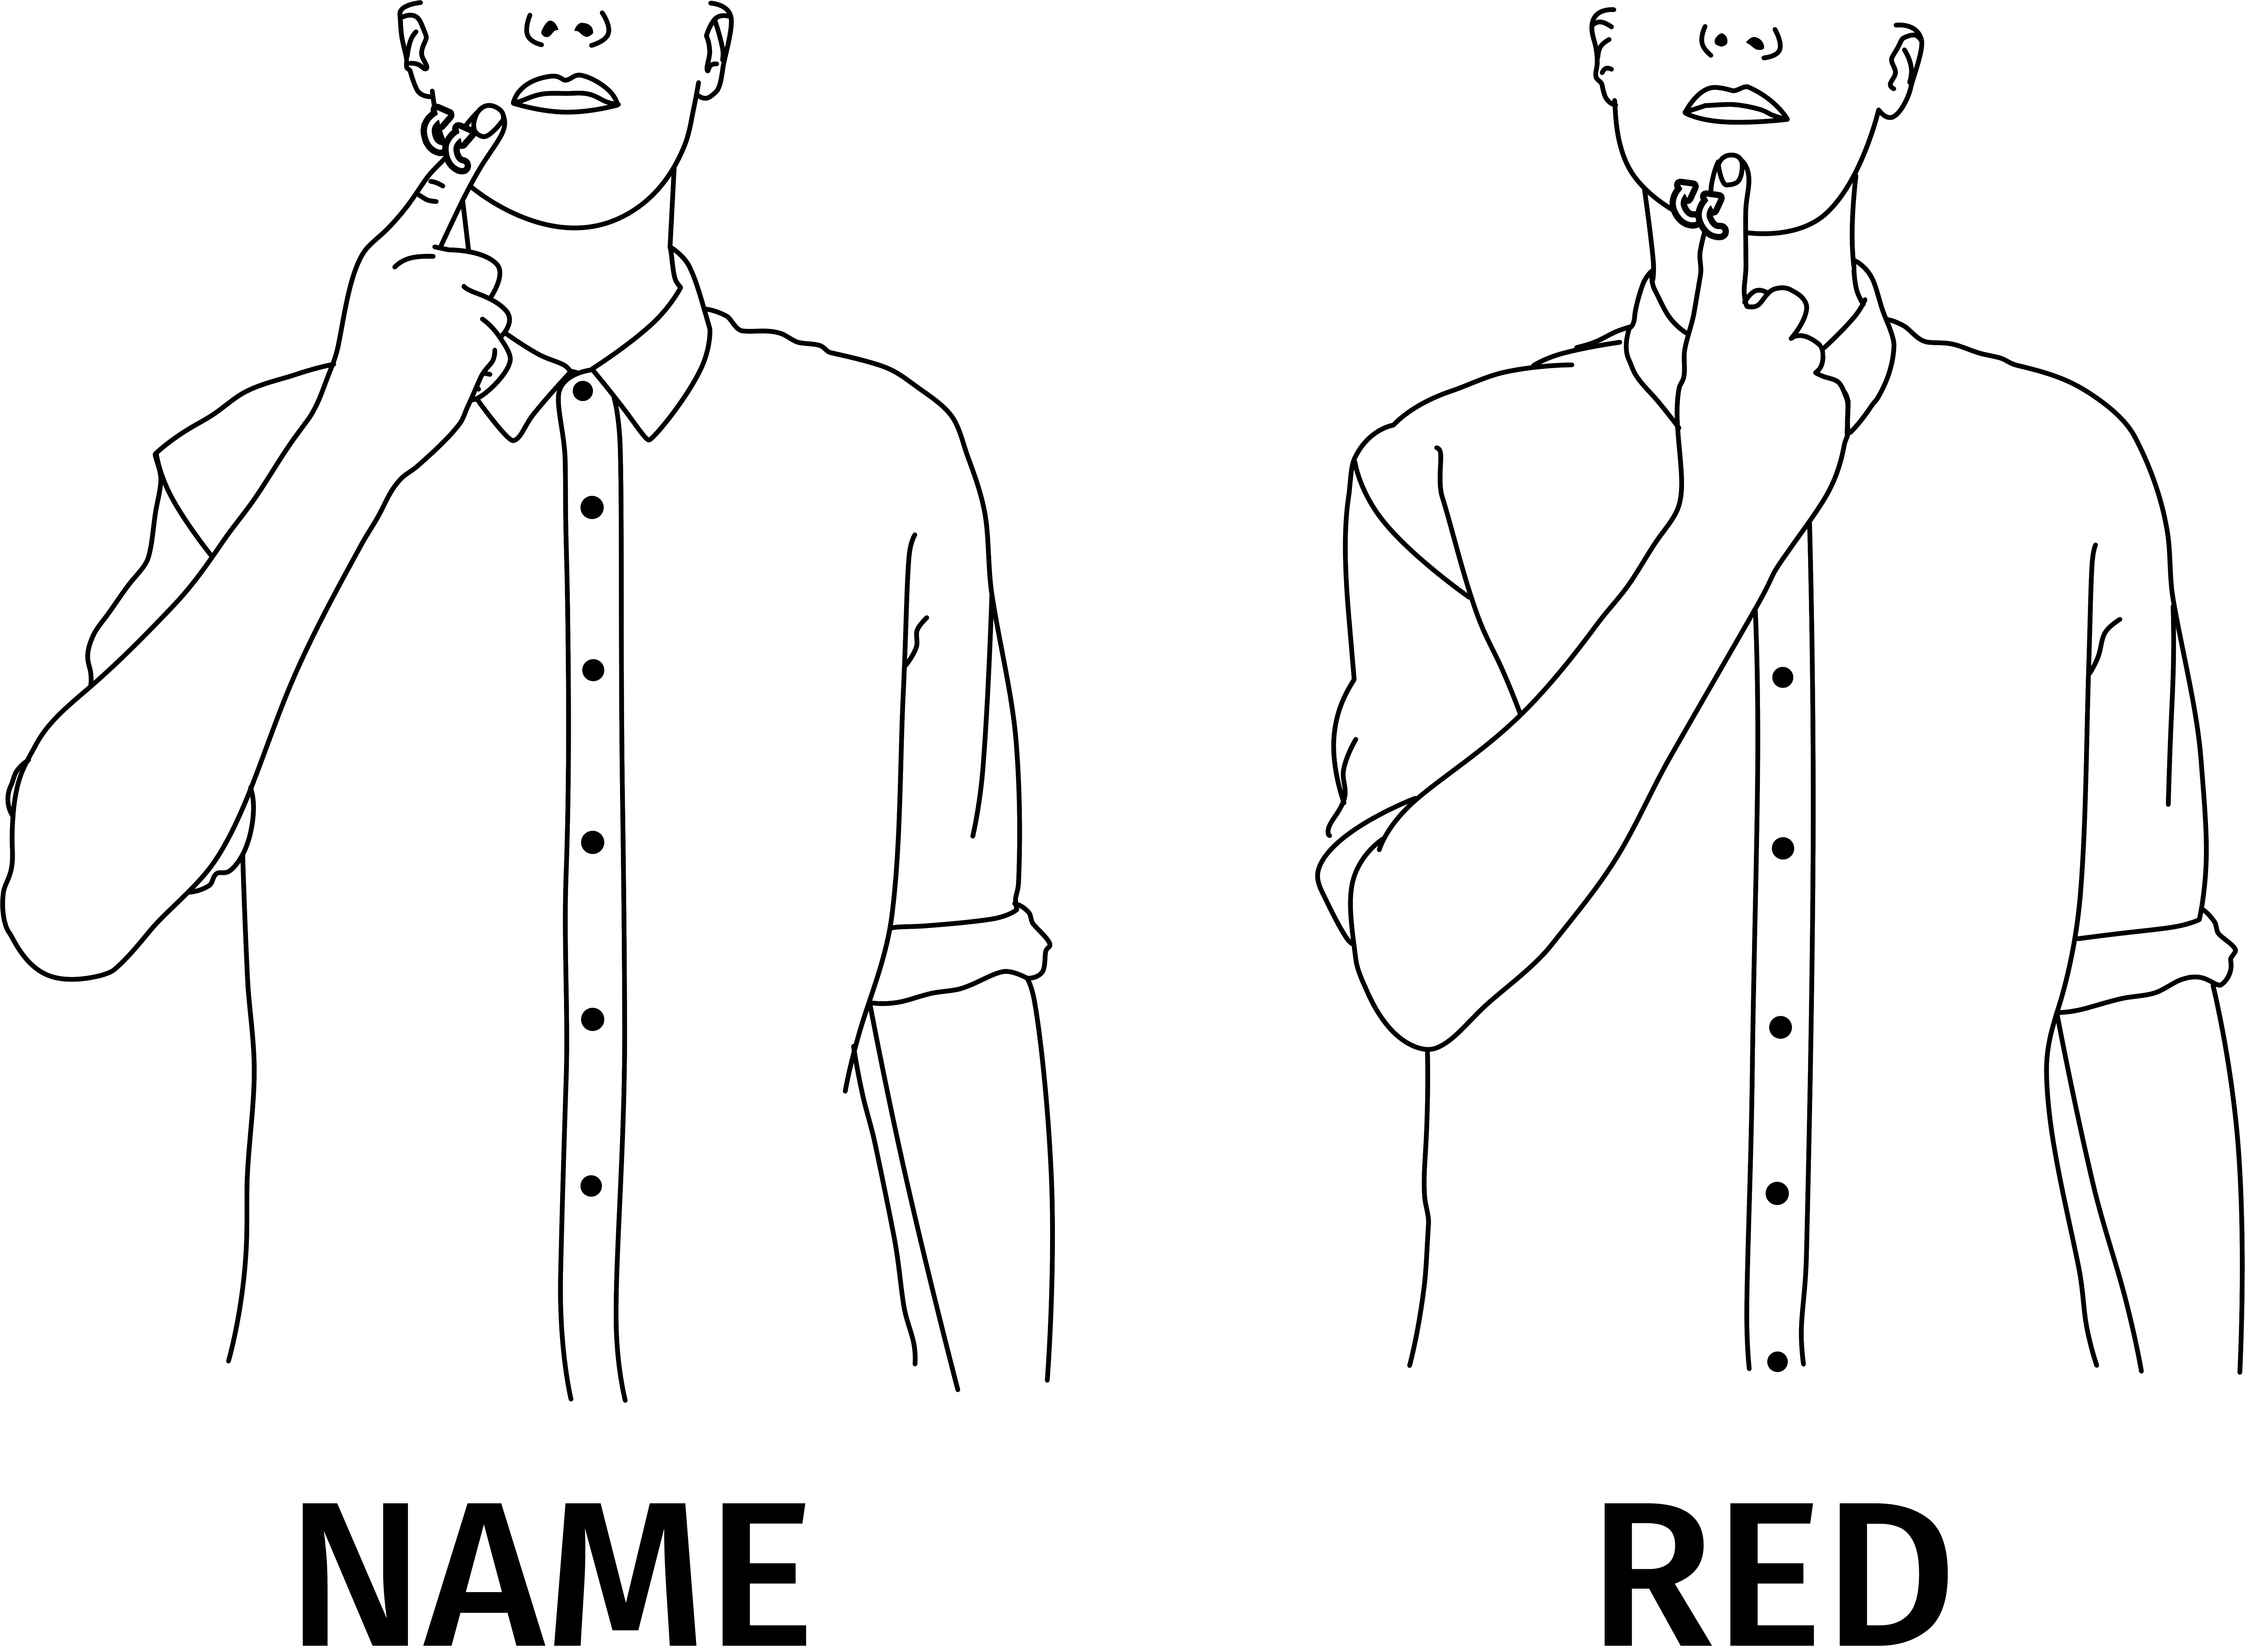
\includegraphics[width=1.0\textwidth]{minimalpair2.jpg}
	\caption{An example of a minimal pair resulting from a change in place of articulation. With one variant of the sign \textsc{name} the signer taps her/his cheek two times with her/his index finger, with the sign \textsc{red} this tapping is executed at the chin.}
	\label{minimalpairtwo}
\end{figure}

The exact same processes underlie morpheme formation in sign languages and this, again, can be shown by creating minimal pairs. Sign languages use a limited number of hand shapes, movement directions, places of articulation (often called `locations'), and palm orientations which all have no meaning by themselves\footnote{ It is sometimes claimed that hand shapes, locations, and movements have meaning by themselves (e.\,g., \citealt[943]{sandler2009sign}). The basis of such claims is the following: an extended index finger, for example, is used as a classifier for human beings in American Sign Language. This, however, does, in my opinion, not mean that this hand shape has a meaning on its own. The same hand shape is found in signs which have nothing to do with human beings, for example, in the sign \textsc{wheelchair}. Claiming that a hand shape, a location, or a movement has a meaning on its own would be similar to claiming that the phoneme /z/ in English has a meaning on its own, just because it can be used as a plural marker in some words (e.\,g., \textit{dog} \ding{212} \textit{dogs}). This, of course, does not exclude the possibility of iconicity at a sublexical level (cf. \citealt{kooij2002phonological,zwitserlood2008morphologybelow}). Thus, it is possible for a sublexical unit to have meaning, but this does not mean that each formational unit has a meaning in every case.} to create morphemes, i.\,e., larger meaningful units \citep{stokoe1960sign, battison1978}. I will give two examples to illustrate that minimal-pair formation leads to similar results as in spoken languages.\is{distinctive features} Comparable to the English minimal pair \textit{cool} and \textit{tool}, the signs \textsc{name} and \textsc{red} only differ in place of articulation in DGS, as shown in Figure \ref{minimalpairtwo}.\footnote{ The variant of the sign \textsc{name} used here also exists in a variant in which the index and the middle finger is used instead of the index finger only.} Both signs are produced by a reduplicated tapping movement of the index finger. The only difference between the two signs is the place of articulation. While \textsc{name} is articulated on the cheek, \textsc{red} is articulated on the chin. We thus can conclude that the cheek and the chin are places of articulation used in German Sign Language serving as distinctive features. 

\begin{figure}[bt]
\centering
	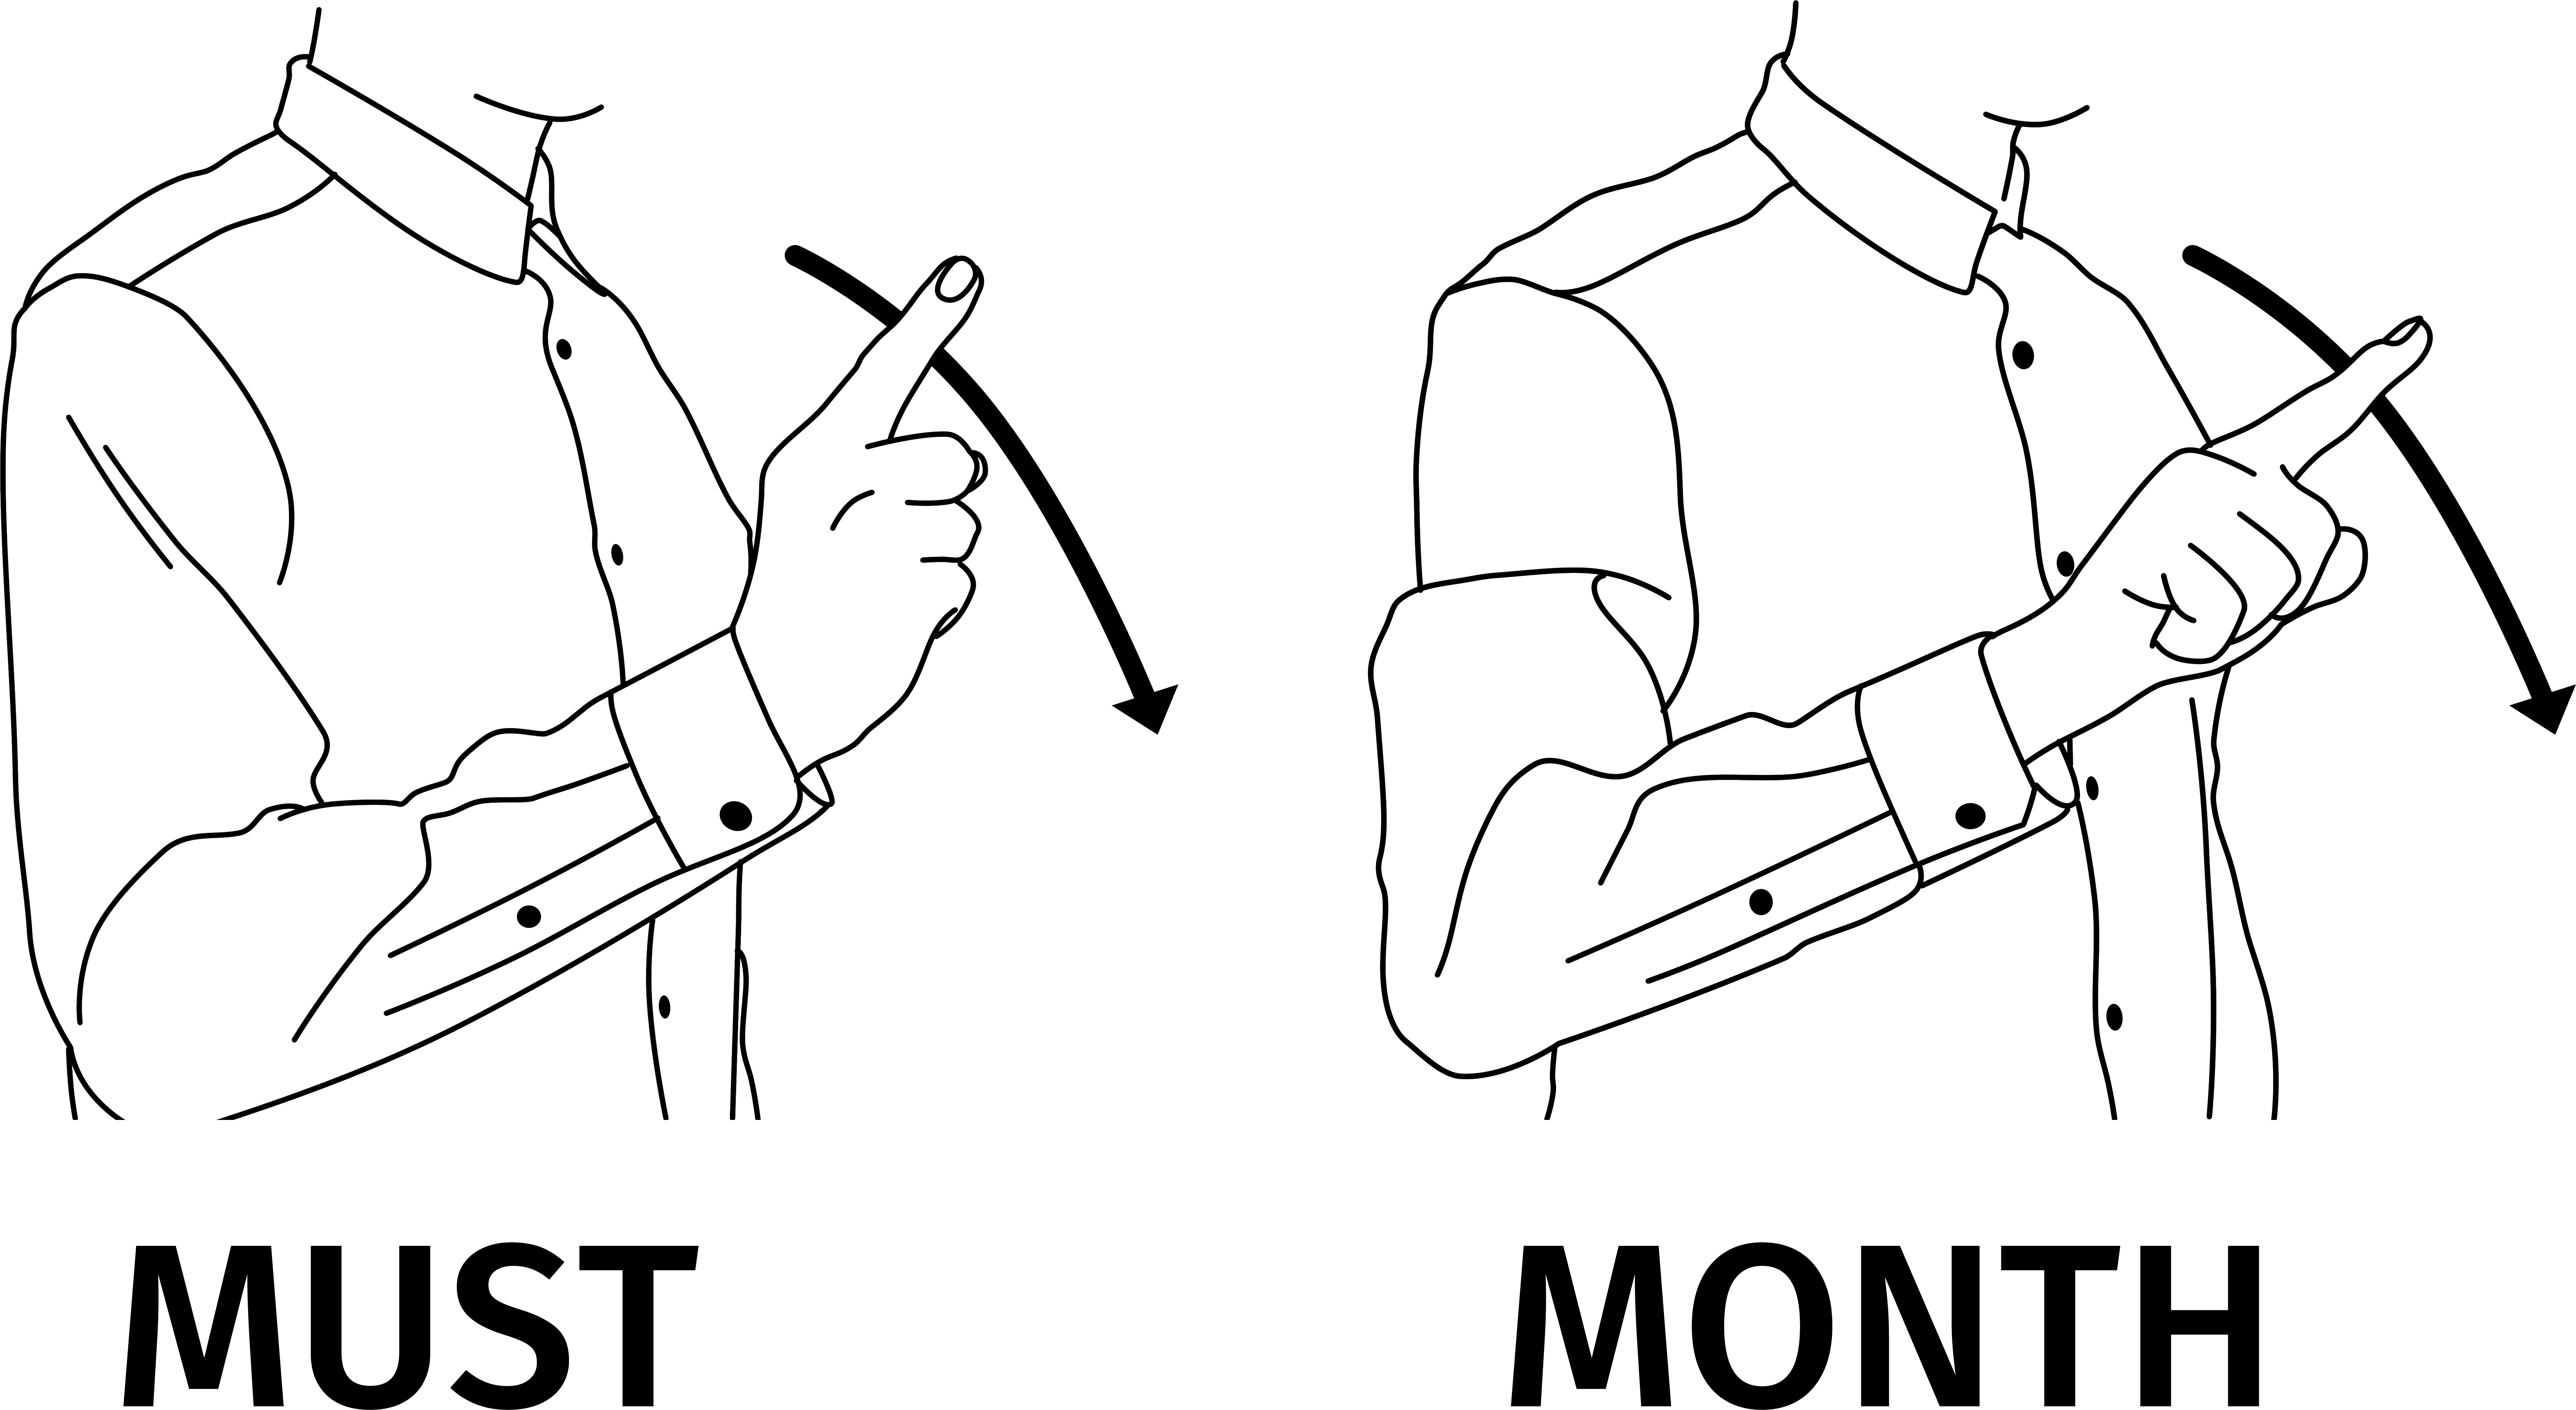
\includegraphics[width=1.0\textwidth]{minimalpair1.jpg}
	\caption{An example of a minimal pair resulting from a change in hand orientation. With the sign \textsc{must} the palm faces sidewards, with the sign \textsc{month} the palm faces downwards.}
	\label{minimalpairone}
\end{figure}

Similar to the shape of the lips, the orientation of the palm is used to create meaning differences. In DGS, for example, the signs \textsc{must} and \textsc{month} only differ in palm orientation. Both signs are articulated by a downward movement of the forearm with the index finger extended.  While \textsc{must} is signed with the palm facing sideways, \textsc{month} is signed with the palm facing downwards, as illustrated in Figure \ref{minimalpairone}. From this, we can conclude that the two palm orientations (sideways and face-down) are used as distinctive features\is{distinctive features} in DGS.

Taken together, besides surface differences, spoken and sign languages use the same mechanism to build meaningful elements by using meaningless distinctive building blocks. 


\is{double articulation|)}

\subsection{Building syntactic structures---embedding and recursion}
Signed and spoken languages are not only similar with respect to double articulation, but on all levels of linguistic description. To give another example, let us take a brief look at embedding and recursion in the syntactic domain. One main feature that has been argued to be fundamental for human languages is that it is possible to take a structure which was produced by applying a syntactic rule and apply the same rule to the structure again (i.\,e., take the output of a rule and use it as the input for the same rule again). In English, for example, we can build a relative clause introduced by \textit{that} (e.\,g., \textit{The beer that I bought in the store was delicious}). The product of the applications of this rule (i.\,e., the relative clause) can now be taken as input for the exact same rule; that is, we can embed another relative clause in the structure (e.\,g., \textit{The beer that I bought in the store, that is now closed, was delicious}). We can thus create a theoretically infinite sentence applying the same rule over and over again. Structure embedding and recursion are major structure-building processes used in natural languages.\footnote{ There are, of course, other possibilities of building recursive structures besides relative clauses in a language, e.\,g., affix stacking of the sort \textit{anti-anti-establishment}, adjective stacking, or all kinds of clausal embeddings.} 

Interestingly, early research on American Sign Language seemed to indicate that similar structures are not possible. In fact, it was claimed that the whole mechanism of subordination was absent in the language as no overt complementizers could be found \citep{thompson1977lack}. However, subsequent research revealed that there are not only relative clauses in sign languages, but that subordination in general is equally possible in this type of language, but only if one knows where to look as subordination is not marked by manual signs, but with non-manual markers in the face \citep{liddell1980american, padden1983action} (for an overview of subordination in sign languages, see, for example, \citealt{gijn2004quest,branchini2014,pfausteinher2016matterofcompl,pfausteinbach2016complexsentences}). In fact, it is not only possible to create relative clauses in sign languages, but they show exactly the same typological variation as spoken languages as both types of languages either used internally-headed relative clauses (e.\,g., American Sign Language; cf. \citealt{liddell1980american} or Italian Sign Language; cf. \citealt{branchini2014}) or externally-headed relative clauses (e.\,g., DGS, cf.  \citealt{pfau2005relative}).\footnote{ The picture in fact is far more complex as sign languages exhibiting internally-headed relative clauses usually also have externally-headed relative clauses (see \citealt{wilbur2017internally} for an overview)---however, not much is known about relative clauses in different sign languages.} And it is, of course, possible, to embed an already embedded structure just like in spoken languages. Although I am not aware of any examples showing that a relative clause can embed another relative clause, it is at least possible to embed a relative clause under another clause as illustrated for American Sign Language in (\ref{ex:relclauseasl}). 

\begin{exe}
\ex American Sign Language \citep[10]{wilbur2017internally}\\ %{\hspace{8pt}top} {} {\hspace{221pt}br} {}  \\
\slg[top]{dog\textsubscript{i}} \slg{index\textsubscript{1} see} \slg[br]{that john say mary chase} $t$\textsubscript{i} \slg{that}
% {$\overline{\textrm{\textsc{dog}\textsubscript{i}}}$} {\textsc{index}\textsubscript{1} \textsc{see}}  {$\overline{\textrm{\textsc{that john say mary chase } \textit{t}\textsubscript{i}}}$} {\textsc{that}}
\glt `I saw the dog that John said that Mary chased.' \label{ex:relclauseasl} 
\end{exe} 

\noindent It is of course nevertheless possible to embed a structure in a structure of the same kind in sign languages. Such a case of real recursion is shown in the DGS example in (\ref{ex:recursion}).\footnote{ The glosses `right' and `left' indicate that the signer turns his/her body and signs the respective signs on the sides of his/her body.}

\begin{exe}
\ex \slg[left]{laura think} \slg[right]{fabian think} \slg{otto sick}
%{\hspace{47pt}left} {\hspace{49pt}right} {}  \\
 %{$\overline{\textrm{\textsc{laura think}}}$} {$\overline{\textrm{\textsc{fabian think}}}$} {\textsc{otto sick}}
\glt `Laura thinks that Fabian thinks that Otto is sick.' \label{ex:recursion}
\end{exe} 

\noindent Taken together, sign languages are natural languages with the same general architecture on all levels of linguistic description, as exemplarily shown for the phonological building processes and embedded structures. In the next section, I will discuss the role of non-manual markings and then present some basic facts about and properties of German Sign Language. Finally, I will discuss the data sources used for the present study.

\section{The role of non-manual markings}\label{sectionnmms}
\is{non-manual markings|(}
Since the very beginnings of sign language linguistics, namely since the seminal work on American Sign Language by William Stokoe, it has been assumed that non-manual markings, produced simultaneously with the manually signed lexical items, are the ``key to syntactical structure'' \citep[63]{stokoe1960sign}. Research since then has indeed shown that non-manuals, such as eye-gaze, movements of the eyebrows, the head, the upper body, or the shoulders, are cross-linguistically used for syntactic purposes. Examples of constructions which are encoded non-manually in sign languages include topicalizations (e.\,g., \citealt{aarons1994aspects, aarons1996topics,brunelli2011antisymmetry}), interrogative constructions (e.\,g., \citealt{neidle2000syntax}; \citealt{zeshan2004interrogative}; \citealt{zeshan2006negative}; \citealt{brunelli2011antisymmetry}), negation (e.\,g., \citealt{pfau2002applying, roland2002v, zeshan2004negation, zeshan2006negative}), subordination (e.\,g., \citealt{wilbur1999syntactic, pfau2005relative, cecchetto2006strategies, branchini2009relatively}, tense \citep{zucchi2009along}, or epistemic modality \citep{bross2017scope}. For an overview of the use of non-manuals see also \citet{pfauquer2010nonmanuals}.

Non-manual markings often---but not necessarily---are grammaticalized gestures which can also be observed as speech-accompanying gestures in spoken languages (e.\,g., \citealt{wilcox2004gesture, pfau2006modality, pfau2011grammaticalization}). That such non-manual markings, such as eyebrow raise or head shakes, are not gestures anymore, but parts of the grammar of a sign language can be shown in different ways. The most obvious difference between a gesture and a non-manual marker is its scope and timing. Non-manuals align to well-defined constituents of signed clauses and exhibit clear on- and offsets while the scope and timing of gestures is much more free (e.\,g., \citealt{bakershenk1983, emmorey1999signers, wilbur2003modality}). Additionally, it has been shown that while facial gestures are processed in the right hemisphere, grammatical non-manual markers of the face are processed in the left hemisphere, as would be expected for linguistic signals \citep{corina1989recognition}. Consequentially, right hemishperic brain lesions can lead to impairments of affective, but not grammatical facial expressions \citep{kegl1991interplay, poizner1992neural, loew1997fractionation, corina1999neuropsychological}. The other way around is also true: lesions in the left hemisphere lead to an impairment of grammatical, but not affective facial expressions \citep{kegl1997crosslinguistic}.

It is often assumed that non-manual markers in sign languages are equivalent to intonation in spoken languages (e.\,g., \citealt{sandler1999prosody}). This is plausible as both are suprasegmental structures. Additionally, both are used for similar functions. For example, all sign languages studied so far use non-manual markers, usually an eyebrow raise, to indicate polar interrogatives. Similarly, intonation is often used to mark polar interrogatives in spoken languages. However, not all non-manuals are similar to intonation in this respect. A head shake, frequently used in sign languages to mark negation, for example, can hardly be equated with intonation as suprasegmental means are rarely used in spoken languages to mark negation.

While the comparison of non-manual markings to intonation is a purely phonological claim, on the syntactic side it has been argued that non-manuals are ``frequently associated with syntactic features residing in the heads of functional projections'' \citep[43]{neidle2000syntax}. Additionally, it was often assumed that the spread of the non-manuals marks their c-command domain and that the greatest intensity of the non-manual markers is at its position of origin (\citealt{bahan1996}; \citealt{petronio1997}; \citealt[43--45]{neidle2000syntax}; \citealt[311--312]{sandler2006sign}).\footnote{ Note that this is not the case with topicalizations as non-manuals only mark the topic, but not the whole clause in the c-command domain.} Concerning the hypothesis that non-manuals are associated with head features, I will defend the view that non-manuals are not (necessarily) themselves syntactic heads, but rather reflexes of Spec-head agreement. I will call this the `Non-Manuals as Syntactic Markers Hypothesis':

\begin{exe}
\ex \textit{Non-Manuals as Syntactic Markers Hypothesis:}\\
Non-manuals do not spread uniformly across constituents, but have an intensity peak at some point. This point, the intensity peak of the non-manuals, marks the location of a syntactic head triggering the non-manuals via Spec-Head agreement. Additionally, the spread of the non-manuals may mark the c-command domain of this head. \label{nmasmh}
\end{exe}

\noindent If Neidle and colleague's (\citeyear{neidle2000syntax}) claim that non-manuals spread over the c-command domain of the head triggering them is correct, it is interesting to note that different non-manual markers are generally assumed to have different spreading domains regarding their location on the signer's body. For non-manuals produced with the face, for example, it has often been noted that a general split exists between non-manuals produced with the upper and those produced with the lower face. While upper-face non-manuals seem to be associated (cross-linguistically) with larger domains and usually fulfill syntactic functions, lower-face non-manuals have a smaller spreading domain and are usually associated with one phrase (e.\,g., \citealt{liddell1980american, coerts1992nonmanual, wilbur2000phonological, wilbur2003modality, brentari2002prosody}). \citet[249]{wilbur2009productive}, for example, notes: 

\begin{figure}[bt]
\centering
	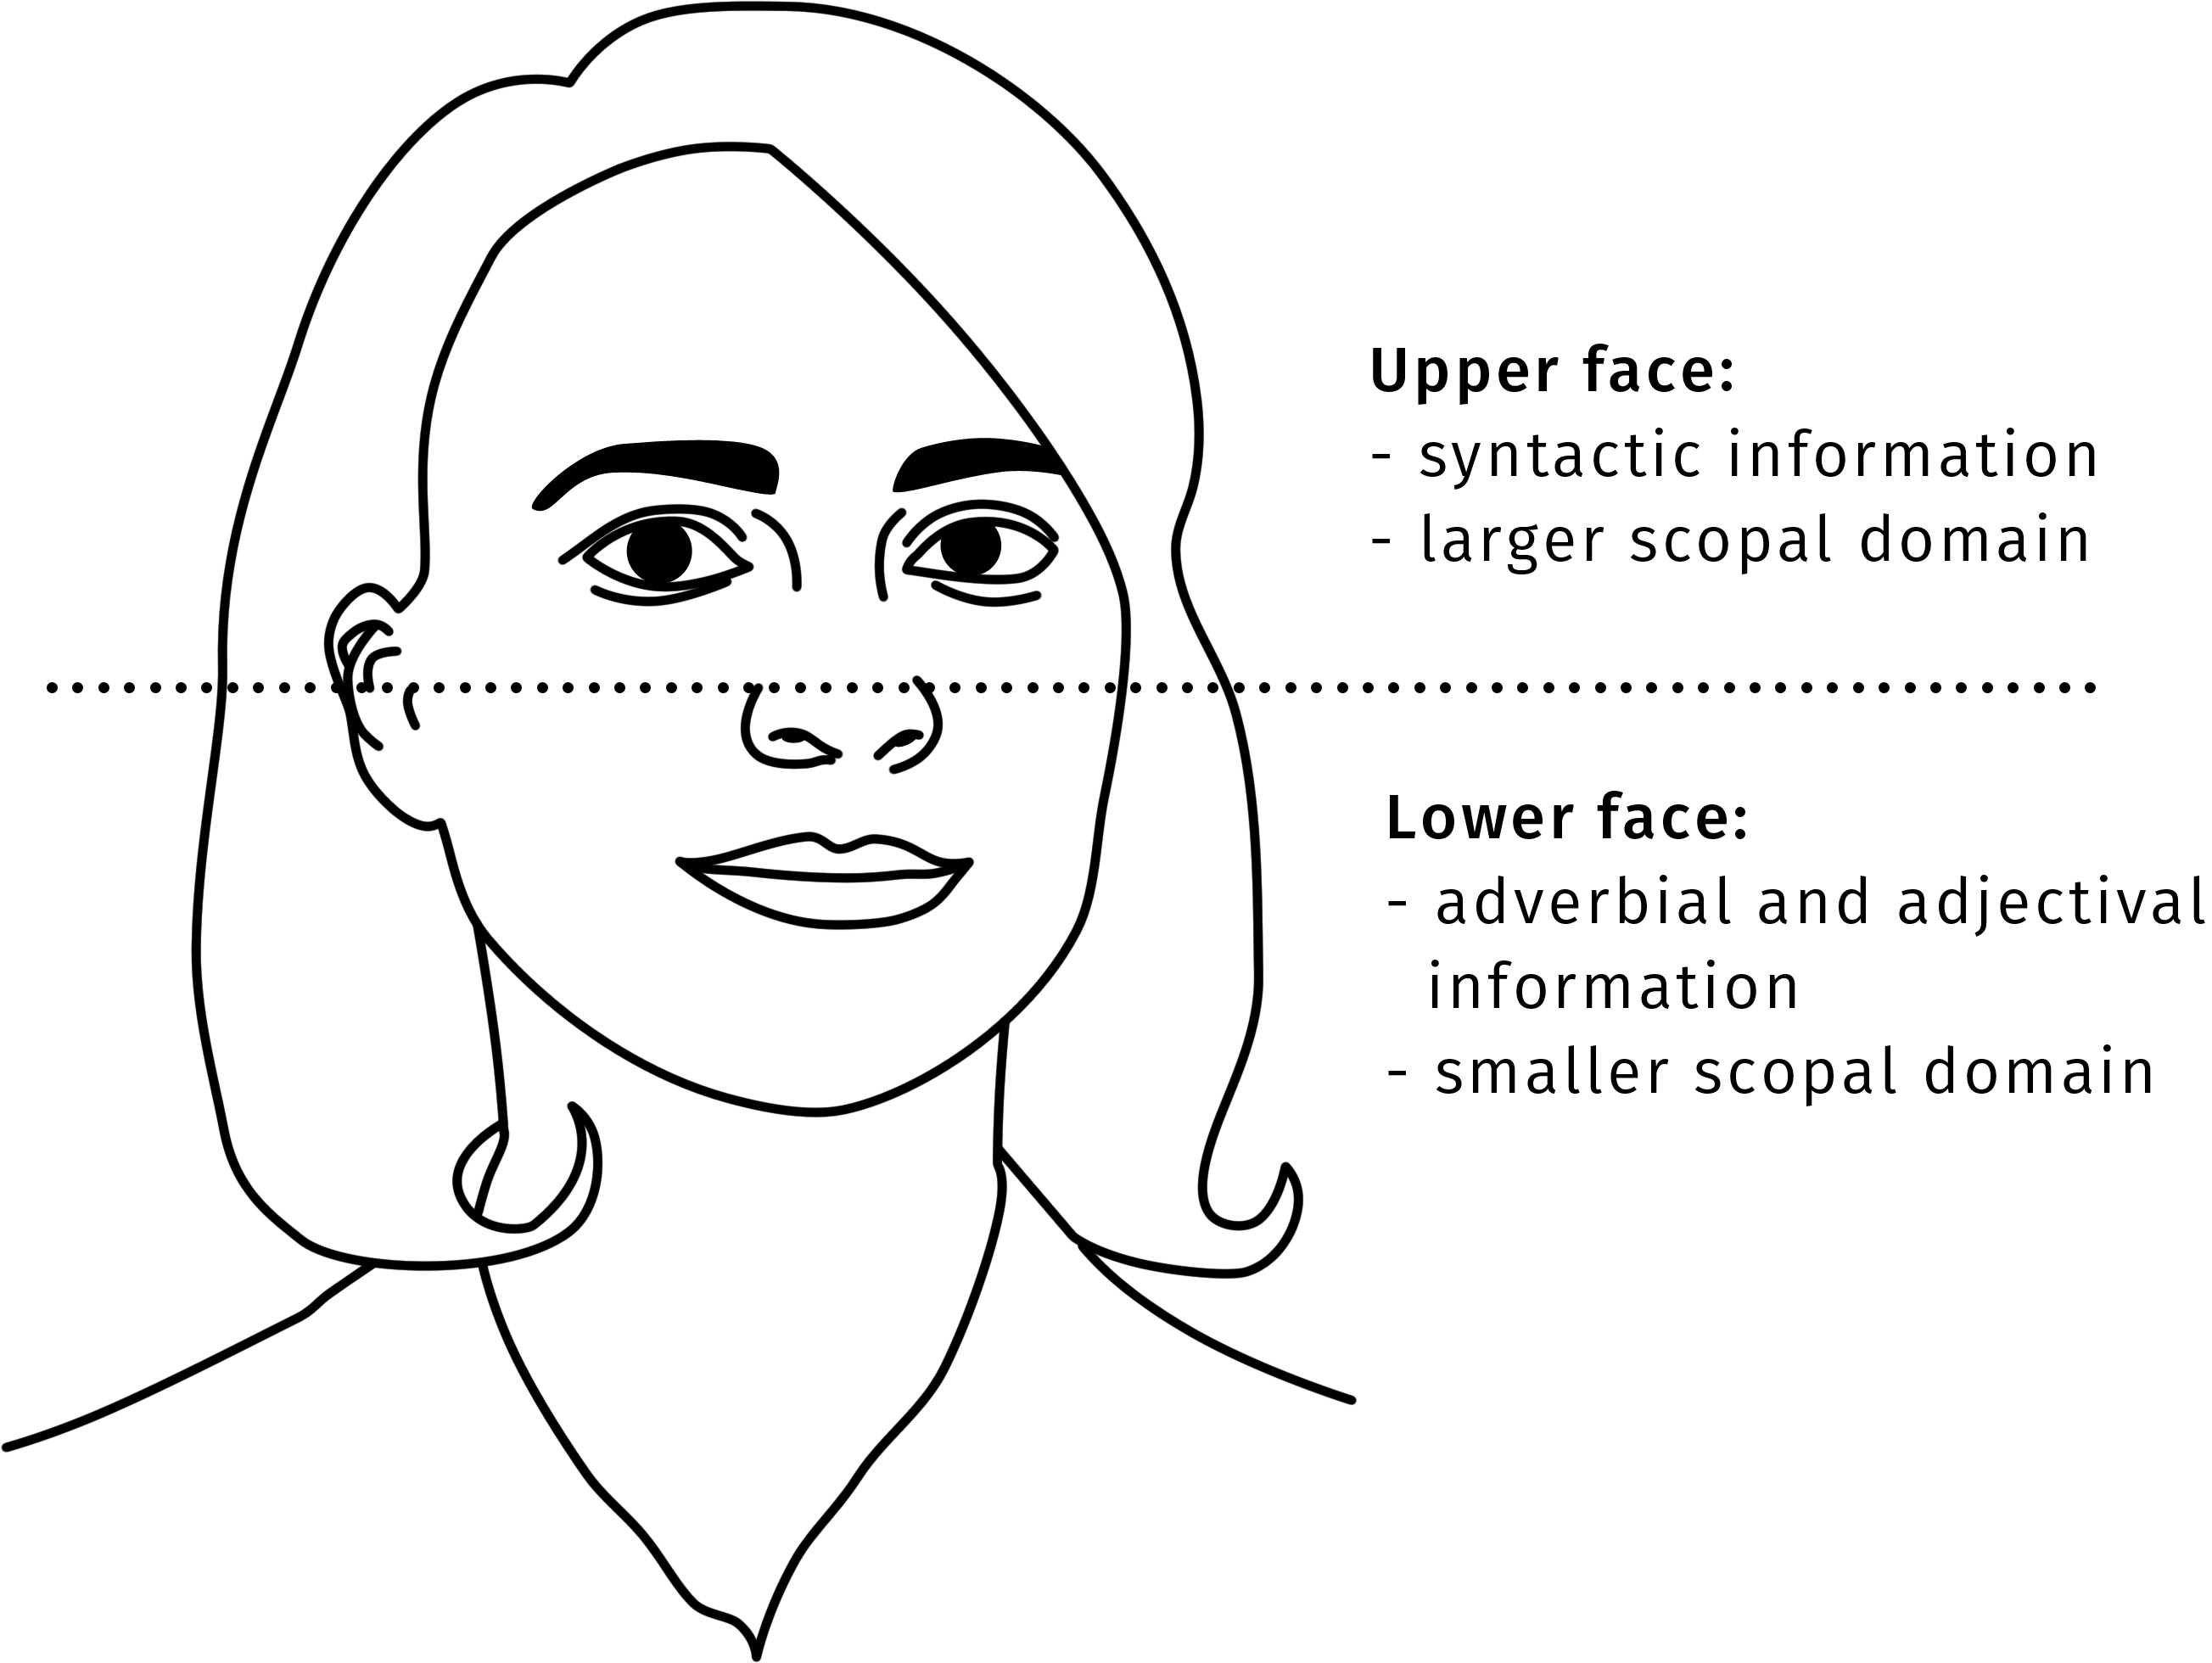
\includegraphics[width=1.0\textwidth]{face.jpg}
	\caption{The division of labor of the upper and lower face found in many sign languages.}
	\label{upperlowerfacedivisionoflabour}
\end{figure}

\begin{quote}
The lower part\label{wilburquote} of the face tends to produce meaningful markers (adjectives, adverbs) that associate with specific lexical items or phrases with those lexical items as heads (e.g., N or NP, V or VP). The upper part of the face (eyebrows, head position, head nods, eyegaze) tends to co-occur with higher syntactic constituents (clauses, sentences) even if such constituents contain only a single sign (e.g., a topicalized noun). 
\end{quote}

\noindent This general split between the upper and lower face is illustrated in Figure \ref{upperlowerfacedivisionoflabour}. See also the main hypothesis underlying the present study discussed in Section \ref{hypotheses}.


It has to be noted that non-manual markers usually come in bundles. It would be desirable to identify one marker for a specific function, for example, eyebrow raise for marking a polar interrogative. However, it turns out that this is often a very hard task, although it has been repeatedly proposed that non-manual markers combine compositionally (e.\,g., \citealt{nespor1999prosody, sandler2006sign, dachkovsky2009visual, herrmann2013modal}). I will describe this problem in more detail for questions which are not only marked by eyebrow movements in DGS, but additionally by putting the head forward and tilting it sideways in the Sections \ref{polarinterrogativesdgs}, \ref{whinterrogativedgs}, \ref{rhetq}, and \ref{perhapsmoodirrealis} and show that such a compositional analysis is indeed possible. I will argue that the eyebrows are used to clause-type a sentence, that the head is put forward to indicate that an answer or other reaction is expected, and that sideways head tilts are used to express the degree of epistemic commitment.





\is{non-manual markings|)}


\section{German Sign Language}\label{basicclausstructuredgs}


German Sign Language (\textit{Deutsche Gebärdensprache}, DGS) is a sign language used mainly in Germany. The number of DGS users can only be estimated. A frequently cited number is 80\,000. This number, however, is only an estimation of the amount of deaf people in Germany (e.\,g., \citealt{dgb}) which is often equated with the number of deaf sign language users in Germany (e.\,g., \citealt{herrmann2007,schwagerzeshan2010}). However, it is in fact not exactly clear how many deaf individuals there are in Germany. The Federal Office of Statistics, for example, estimates that there are around 28\,000 deaf people without cognitive impairments living in Germany \citep{schwerbehindertenstatistik2017}, a number that is much smaller than the usually cited 80\,000. Of course, not all deaf people might use sign language and there are also hearing people using DGS. Finally, many hard of hearing individuals also use DGS and the number of hard of hearing individuals is much higher than the number of deaf people. The Federal Office of Statistics assumes that there are over 250\,000 hard of hearing people living in Germany \citep{schwerbehindertenstatistik2017}. Thus, on some estimates, the number of DGS users is much higher. The European Union of the Deaf \citep{eud2012} or the Ethnologue \citep{simons2018ethnologue}, for example, assume that there are approximately 200\,000 users of DGS in Germany.

DGS is a rather strict SOV language in both matrix and subordinate clauses (e.\,g., \citealt{keller1998aspekte, pfau2001pseudo}). As would be expected from a SOV language, modal verbs generally appear in a clause-final position, as shown in (\ref{modalverbplacement}) (although there is some variation to the placement of modal verbs as discussed in Chapter \ref{ipsystem}). 


\begin{exe}
\ex \textsc{Elias perform-magic can}
\glt `Elias can perform magic.'\label{modalverbplacement}
\end{exe}

\noindent As DGS is an OV language and as modal verbs occur clause-finally, it is usually assumed that heads of functional projections are to the right (e.\,g.,  \citealt[365]{sandler2006sign}; \citealt[17]{herrmann2013modal}; \citealt[3]{bross2017scope}). This leads to a basic clause structure as represented in (\ref{ex:basciclausstructure}). Note that one of the most controversial topics related to the clause structure of DGS is the question of whether SpecCP is to be located on the left or on the right. I have put SpecCP provisionally on the left in the tree as this is a widely-held opinion (e.\,g., \citealt{herrmann2013modal}) and will discuss the exact position in detail in the next chapter (see Section \ref{whinterrogativedgs}).

\begin{exe}
\ex \label{ex:basciclausstructure}
\begin{tikzpicture}[baseline=(current bounding box.north), scale=0.8]
\tikzset{level distance=35pt,sibling distance=5pt,every tree node/.style={align=center,anchor=north}}
%\tikzset{sibling distance=1pt}
\tikzset{every tree node/.style={align=left,anchor=north}}
\Tree [.CP [.{SpecCP} ] [.{$\overline{\textrm{C}}$} [.IP [.{SpecIP} ] [.{$\overline{\textrm{I}}$} [.VP [.{SpecVP} ] [.{$\overline{\textrm{V}}$} [.{} ] [.{V\textdegree } ] ] ] [.{I\textdegree } ] ] ] [.{C\textdegree } ] ] ]
\end{tikzpicture}
\end{exe}


\noindent In many cases, the SOV order can be altered by fore- and backgrounding processes such as topicalizations. Additionally, word order is affected by the figure-ground principle. I will have more to say about word order in Section \ref{declarativesentences} and discuss topicalizations in Section \ref{topicsindgssection}. 

DGS is a comparatively well-studied sign languages. Consequently, there is a vast literature on many aspects of the language. Besides more descriptively oriented grammars \citep{papaspyrou2008grammatik,happ2014vork} and research from a more applied perspective \citep{eichmannhansenhessmann2012,dumig2013}, works on language acquisition (e.\,g., \citealt{leuninger1997lena,hanel2005spracherwerb,haenelfaul2012erwerb}) or the phonological structure (e.\,g., \citealt{benner2012,herrmann2012prosody,dumig2013}) from various frameworks, there is a huge Generative research tradition. Within this tradition, various topics have been addressed, including negation \citep{pfau2008headshake,pfau2016featural}, relative clauses \citep{pfau2005relative}, agreement \citep{pfau2006thedevelopment,steinbach2007grammaticalization,steinbach2011agreement,pfausalzmannsteinbach2018agreement}, pluralization \citep{pfausteinbach2004}, role shift \citep{hermannsteinbach2012quotation}, or modality \citep{herrmann2007,herrmann2013modal}---to name but a few.

Research on DGS has so far mainly been concentrated on the variants used in the areas in which the big sign language research centers are located---most notably, in Göttingen in central Germany, Hamburg in northern where the DGS corpus project \citep{jahn2018} is hosted, Berlin in north-eastern Germany and in a former center in Frankfurt in south-western/central Germany. The data presented in this book, in contrast, comes from southern Germany. The DGS variant used in southern Germany is very similar to the sign language used in the rest of Germany, although there are some dialectal differences in vocabulary and also some syntactic differences which mainly concern negation and contrastive focus (at least as far as I am aware of), as described in Section \ref{contrastivefocussubection} (see page \pageref{contrastivefocus}) and Section \ref{imperativesindgs} (see page \pageref{negationnegaation}) respectively. 

%\clearpage

\section{Data sources}\label{methods}
The data presented in this book were elicited from nine native signers of German Sign Language living in the states of Bavaria (six individuals) and Baden-Württemberg (three individuals) in southern Germany. Eight of them are deaf and one is a hearing child of deaf adults (CODA). Six of the signers acquired sign language from birth, three are early learners, defined as individuals who started acquiring sign language before the age of four (one acquired DGS since the age of two, one at the age of one and a half, and one since the age of three). Additionally, data from two late-learners were collected. Both late learners are deaf from birth and visited deaf schools, but reported that they did not use German Sign Language, but manually coded German in school. The age range of the signers was between 20 and 56, the mean age was 28.44.60 (\textit{SD} $=$ 6.04), four of them were men. It was ensured that all consultants had proficient written language skills and all of them had at least a high-school diploma (a German \textit{Realschulabschluss}). 



The data were elicited in face-to-face interactions which were recorded on video. There was a total of 16 sessions. Each session lasted for about 2 hours. Consultants received the (written) material to be discussed one week before the video recordings to familiarize themselves with the meanings of the sentences. At the actual recording sessions, the sentences (or mini-dialogues) were presented on sheets of paper. In many cases, the sentences were presented with context sentences to arrive at the desired reading. Each sentence was presented to them for a few seconds. The consultant read the sentence and had some time to think about its meaning. Then the sheet of paper was covered up. After the sentence was covered up, the consultants again had some time to think about the meaning of the sentence. 

Then they signed what they thought was the best way to express this meaning in German Sign Language. This procedure was chosen to prevent the  signers  from  being  influenced  too  much  by  the  sentence's  written  structure. All translations were videotaped. In many cases, after the sentence was signed, the sentence and possible paraphrases were discussed. Additionally, the  consultants often were explicitly asked for grammaticality judgments (or rather acceptability ratings). Examples of sentences with contexts (in brackets) are given in (\ref{examplematerial}) (of course, the original sentences were in German). The contexts ensure that the example in (\ref{examplemateriala}) receives a deontic and the sentence in (\ref{examplematerialb}) an epistemic interpretation, respectively.

\begin{exe}
\ex\label{examplematerial}\begin{xlist}
\ex (Paul's parents are strict). Paul must be at home at 8 o'clock. \label{examplemateriala}
\ex (The light in Paul's room is on.) Paul must be at home. \label{examplematerialb}
\end{xlist}
\end{exe}

\noindent In line with previous studies (e.\,g., \citealt{herrmann2013modal}), it turned out that signers used manual modal verbs (in this case the sign \textsc{must}) in deontic examples like the one in (\ref{examplemateriala}), but did not use manual modal verbs in epistemic examples like the one in (\ref{examplematerialb}). Instead, sentences with epistemic meanings are marked non-manually with a squint (see Section \ref{sectionepistemic} for more details). Signers were then asked if the examples could be signed without the non-manuals or by adding a manual modal verb. Usually, this was done by repeating the example with the aforementioned changes by the author. Examples including deontic modals did not receive non-manual markings spreading over the whole clause, but the manual modal signs themselves were sometimes marked non-manually (in the case of deontic necessity modals: increased signing speed of the modal verb, lowered and squinted brows accompanying the modal). Again, signers were asked if the sentence could be signed without the non-manuals, while still being acceptable and conveying the relevant meaning. In some cases, it then turned out that the non-manuals were not obligatory, as with deontic modality, in other cases, as in sentences with epistemic meanings, the non-manuals cannot be omitted without a change in meaning. 

The signed sentences were cut into separate video files using Adobe Premiere Pro CC. Each file was annotated for the relevant category (e.\,g., deontic modality). On the whole, this resulted in 1229 video files. The subsequent analysis was not a quantitative, but an incremental qualitative one. The available videos of each category at one point in time were compared, for example, concerning the non-manuals on different levels (upper face, lower face, head movements) to filter out idiosyncrasies of single signers. Remaining questions were used as a departure for the next data elicitation sessions. In the case of polar interrogative sentences, for example, it turned out that the consultants raised their eyebrows, put their heads forward and to the side (see Section \ref{polarinterrogativesdgs} for details). While the eyebrow raise was consistently used by all consultants, putting the head forward and putting it to the side was not present in all instances. After consulting the literature on questions, it was hypothesized that each of the non-manuals would fulfill a specific function. Functions hypothesized to be present were, for example, (i) that the signer does not know the truth of the proposition expressed, (ii) that the signer wants to know the truth value of the proposition expressed, or (iii) that the signer believes that the interlocuter being asked knows the truth about the proposition embedded in the question (e.\,g., \citealt[4]{dayal2016questions}). Subsequently, examples (minimal pairs, if possible) were created in which one function was missing. In the case of polar interrogatives, rhetorical questions were, for example, elicited to scrutinize what happens if the signer does not expect an answer.

One potential problem with this kind of data elicitation is that the signers could be influenced by the grammatical structure of the German sentences. Although such concerns have to be taken seriously, the fact that many of the constructions discussed in this book differ drastically from spoken German can be taken as a strong indication that the influence of spoken German was at least not very substantial (see \citealt[281]{cecchetto2009another} for a similar argument).

Another problem relates to the tension between what \citet[26]{zyman2012two} called the ``breadth approach'' and the ``depth approach''. When investigating a linguistic phenomenon P in a language L the researcher either collects the same judgments from a large number of native speakers of a language (the breadth approach) or collects different judgments from a smaller number of native speakers (the depth approach). While the breadth approach has the advantage of being more precise, it comes with the cost that P can be investigated in less detail. The depth approach, in contrast, has the disadvantage of being less precise in which aspects of P may be subject to inter-speaker variation, but it has the advantage of enabling the researcher to get a broad picture of P and its subphenomena.

As this book is concerned with a large number of different categories and how they combine it was not possible to collect judgments for each example presented from each consultant. I thus adopted the depth approach to study the clause structure of DGS in more detail. Nevertheless, care was, of course, taken so that each judgment was confirmed by several signers. However, it has to be stressed, as \citet{zyman2012two} also notes, that both approaches need to be persued as they complement each other. I am thus convinced that many of the phenomena discussed in this book need to be studied in more detail in the future. 

The same is, of course, true of the spoken language examples presented in this book which are not taken from the literature. I consulted two native speakers of Turkish, two Mandarin native speakers, and three native speakers of the Northern Italian dialect spoken in Sommacampagna (Custoza) to collect acceptability indications for these examples.



\section{Outline of the book}\label{outlinesection}
The present book consists of three main chapters reflecting the three main layers of the clause, the CP, the IP, and the VoiceP layer. Each section in all three chapters basically has the same structure. I will first generally introduce the phenomenon under discussion by briefly sketching what is known about it in spoken languages. Then, I will sketch what the literature has to say about the phenomenon in sign languages and finally discuss my own DGS data. 

In Chapter \ref{cpchapter} I will discuss the CP system of DGS. After a discussion of topic and focus marking in DGS I will describe how DGS encodes different sentence types. Besides the main sentence types, declaratives, polar and constituent interrogatives, as well as imperatives, the chapter will also be concerned with some minor sentence types, namely alternative questions, degree questions, tag questions, suggestive questions, rhetorical questions, and optatives. In Chapter \ref{ipsystem} I will go through the categories discussed in \citet{cinque1999adverbs, cinque2006restructuring}. Some of these categories are located above tense and thus could be considered to still belong to the CP system. The majority of categories, however, are located below tense, but above the VoiceP. In Chapter \ref{insidevp} the remaining Cinquean categories below the VoiceP layer will be discussed. Finally, in Chapter \ref{chapterconclusions}, I will conclude the findings.

